
%%%%%%%%%%%%%%%%%%%%%%%%%%%%%%%%%%%%%%%%%%%%%%%%%%%%%%%%%%%%%%%%%%%%%%%%
\chapter{Spacial Analysis}
%%%%%%%%%%%%%%%%%%%%%%%%%%%%%%%%%%%%%%%%%%%%%%%%%%%%%%%%%%%%%%%%%%%%%%%%

%%%%%%%%%%%%%%%%%%%%%%%%%%%%%%%%%%%%%%%%%%%%%%%%%%%%%%%%%%%%%%%
\section{Introduction to Spacial Analysis}

% nmot difference between last section and this section, were gonna focus a lot more on environment os buckle up
In \autoref{sec_probsnstat}, ambient noise was split into three distinct acoustic environments in order to asses the overall attributes of each. With the numerical attributes of each environments differing by frequency, it is likely the causes and drivers of this ambient noise differ as well. Acoustic forces behind sound under ice are not the same as the primary powers behind sound in an ice free Arctic ocean. \footcite[]{icesound} This section will focus on the relationship between ambient sound under ice and the movement of ice itself.

While looking at a broadband range of frequencies makes sense for a statistical analysis, looking at the spatial correlation of 38 different frequencies on a map would be cluttered. For ease of computing and viewing, the spatial correlation analysis is limited to the frequencies of 300 Hz, 500 Hz, 1000 Hz, and 1500 Hz. 300 Hz, as opposed to 250 Hz, was retained for comparison with the original analysis. While a band around 50 Hz was examined, the low frequencies behaved much differently than most others. This is reflected in the statistic analysis above as the 50 Hz data points are usually different and and it could be assumed the low frequencies have different acoustic drivers. 

A significant amount of this section is a continuation of the work done in a previous iteration of the data in \footcite[]{BonnelMain}. Expanding the frequencies examined in spacial correlation analysis emphasizes that all these frequencies are highly related in both

%%%%%%%%%%%%%%%%%%%%%%%%%%%%%%%%%%%%%%%%%%%%%%%%%%%%%%%%%%%%%%%%%%%%%%%%
% seriouslt why do all my titles sound terrible
\section{Spacial Analysis Methods and Results}
%%%%%%%%%%%%%%%%%%%%%%%%%%%%%%%%%%%%%%%%%%%%%%%%%%%%%%%%%%%%%%%%%%%%%%%%


%%%%%%%%%%%%%%%%%%%%%%%%%%%%%%%%%%%%%%%%%%%%%%%%%%%%%%%%%%%%%%%%%%%%%%%%%%
\subsection{Correlation between Ice Drift and ANL}

Introduce the theory behind 
\begin{enumerate}
\item  ice drift as a vector of speed that we changed into movement/day from EUMETSAT OSIAF
\item  how correlation between ice drift and anl is calculated
\item  the time split up and specific ice condition used
\item 
\end{enumerate}


USE CORRELATION Equation in JASA as well
Questions I want to answer/
 

%%%%%%%%%%%%%%%%%%%%%%%%%%%%%%%%%%%%%%%%%%%%%%%%%%%%%%%%%%%%%%%%%%%%%%%%%%
\subsection{Correlation across Frequencies}
Using the same procedures as in the 'Correlation between Ice Drift and ANL' section

\textbf{Description}
This is a deception of the figure for 1000-1500 Hz on 01dec16-30Jan2017 ice drift and ANL correlation

\textbf{Analysis}
This is the analysis for the ice drift correlation from 01DEC16-30Jan17 for 1000 and 1500 Hz

\textbf{What does this mean?}
this is the what does this mean part for the 1000/1500 spacial correlation analysis

\begin{figure}[h]
\centering
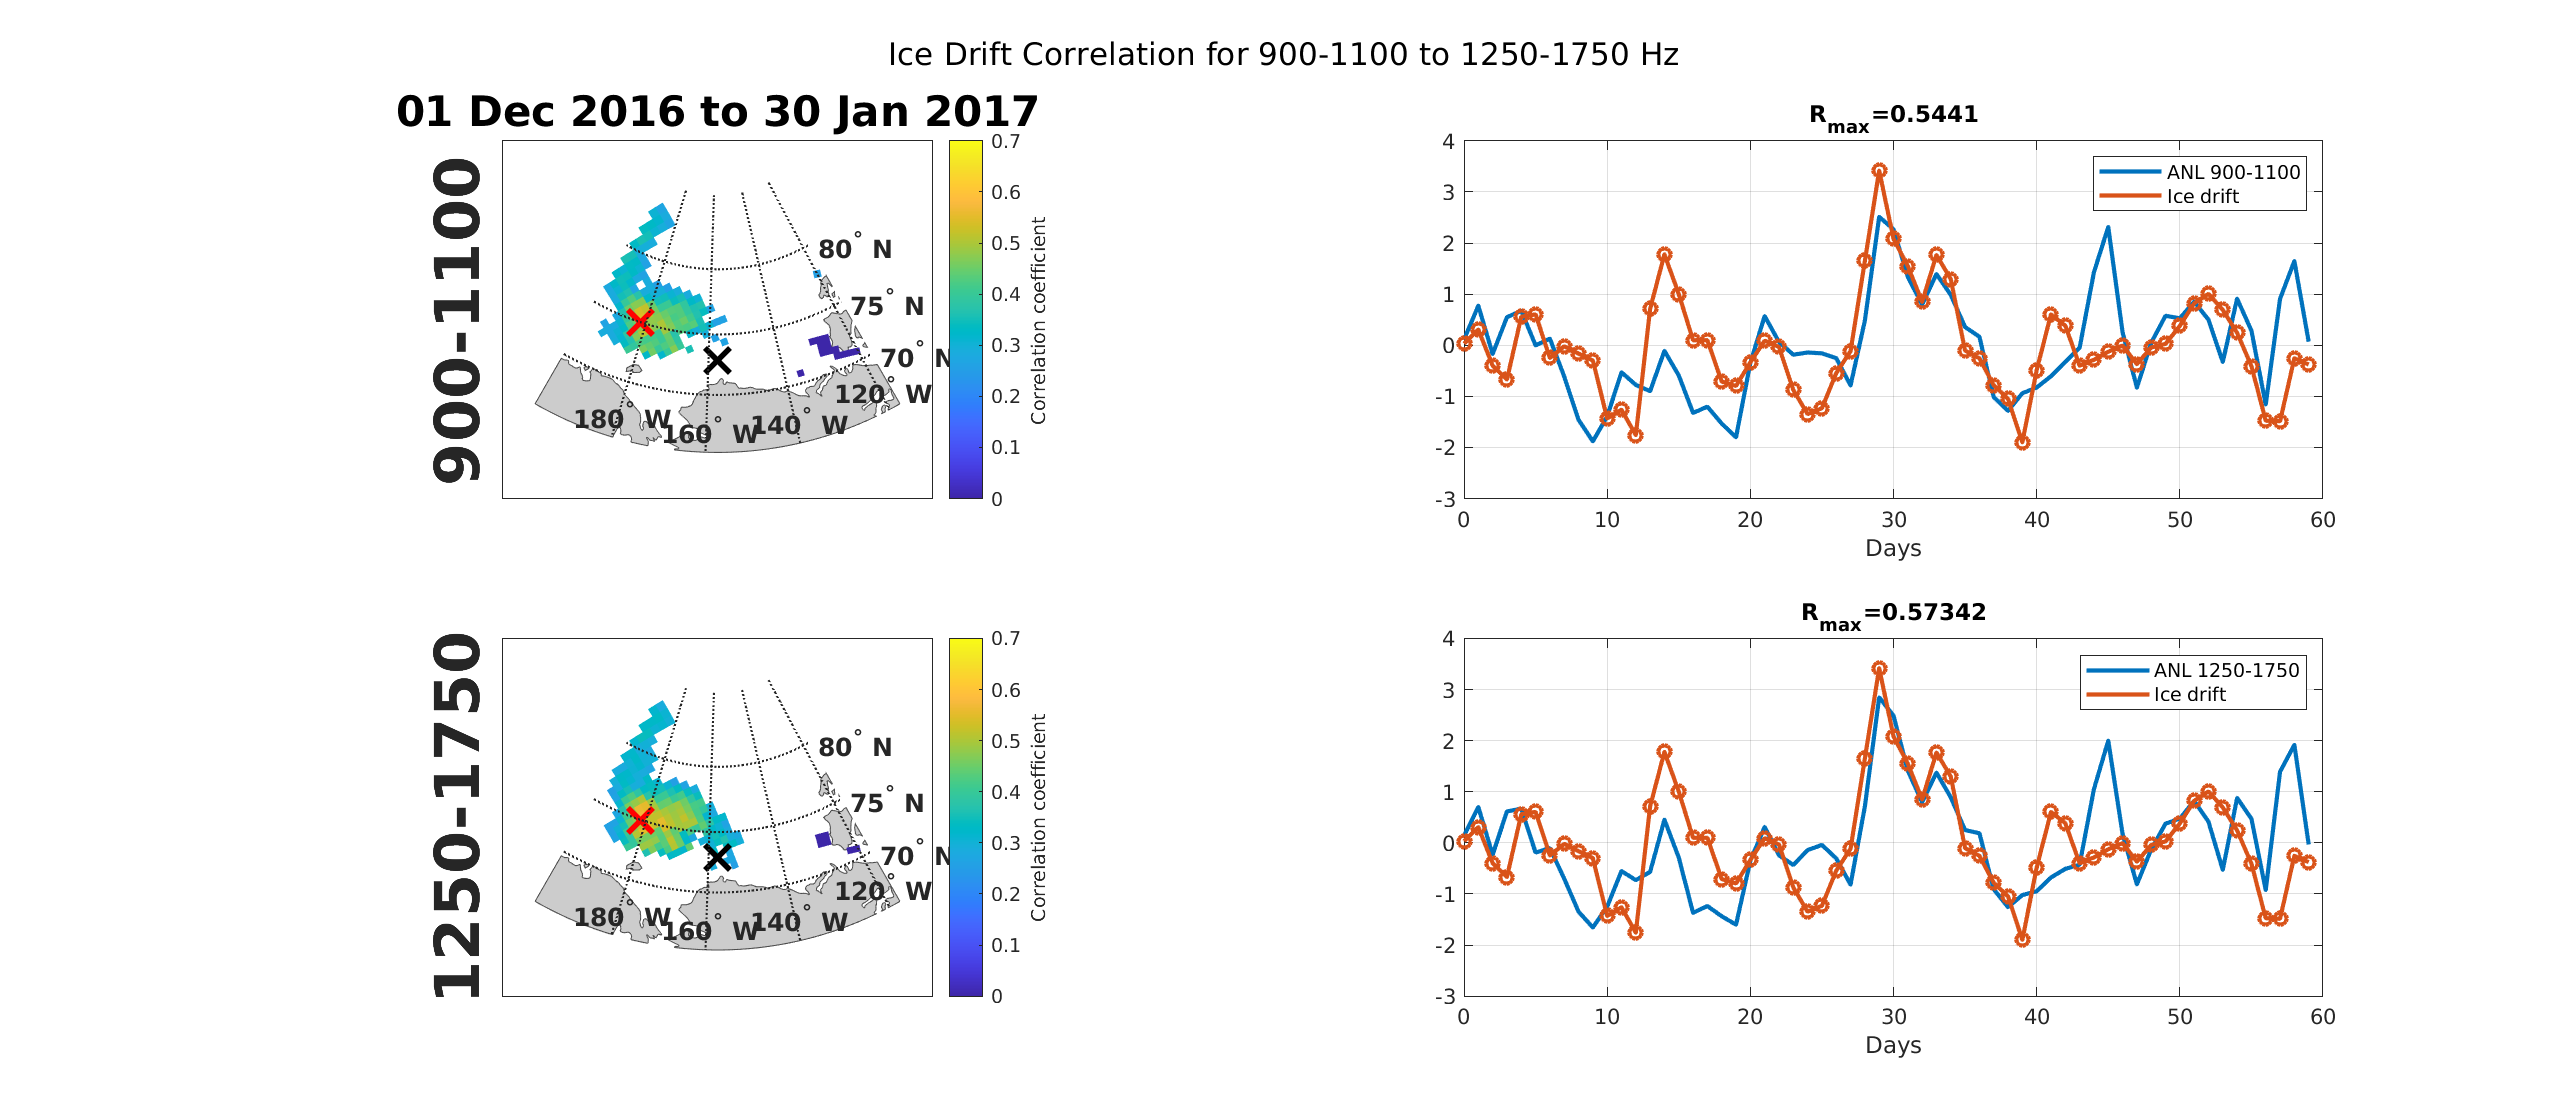
\includegraphics[scale=0.4]{Figures/1000_1500_spatial_corr_20161201-20170130.png}
\caption{Spacial Correlation for 1000 and 1500 Hz 01DEC2016-30JAN2017}
\label{fig_1000_1500corr}
\end{figure}

%%%%%%%%%%%%%%%%%%%%%%%%%%%%%%%%%%%%%%%%%%%%%%%%%%%%%%%%%%%%%%%%%%%%%%%%%%5
\subsection{Correlation across Hydrophones (SHRUs)}

\textbf{Description}
(450-550) 500 Hz is on the top row, (900-1100) 1000 Hz is on the bottom row
The left side/column is the colormap of ice drift correlation
Why are there darkish spots outside the edge area? Because sound comes from here too but is less correlated (0 correlation actually). Another figure (ref fig here) sets a cutoff at 0.4 correlation, removing the 
The blue line is the ANL at that given frequency, which is more continuous than the orange line, which has ice drift per day. Both of these data are normalized to 0 using the ‘z-score’ function of matlab
The maximum correlation value found between the ANL and ice drift is displayed at the top of each time series; this was found using the ‘corr’ function of Matlab. I also saved the p-values but didn’t put them in

\textbf{Analysis}
This particular ice drift correlation graph is for the higher bandwidths of 500 and 1000 Hz, demonstrating that the ANL is present in a large bandwidth of frequencies, from at least 300 up to 1500
The ice drift and ANL z-score levels trend very similarly spiking and dropping at comparatively the same time. Correlation does not equal causation but it suggest that most of the ambient noise under ice comes from the ice moving itself
The red X is not a display of where the sound is coming from, because the sound is coming from everywhere. The red X indicated the point of highest correlation between the ANL and the ice drift. There is literally ice all over, and sound travels through ice as well.

\textbf{What does this Mean?}
This demonstrates the correlation between ice drift and noise level in the arctic across many frequencies, including higher ones
It suggests that under ice ambient noise is related to the movement of the ice itself. ANL mode tends to be around 55 dB, IS THIS HIGHER OR LOWER THAN NORMAL LOOK UP HISTORY
It is very important to not that \textit{ice is more of a line source or a plane source} and modelling as a point source isn't entirely realistic to the environment.

\begin{figure}[h]
\centering
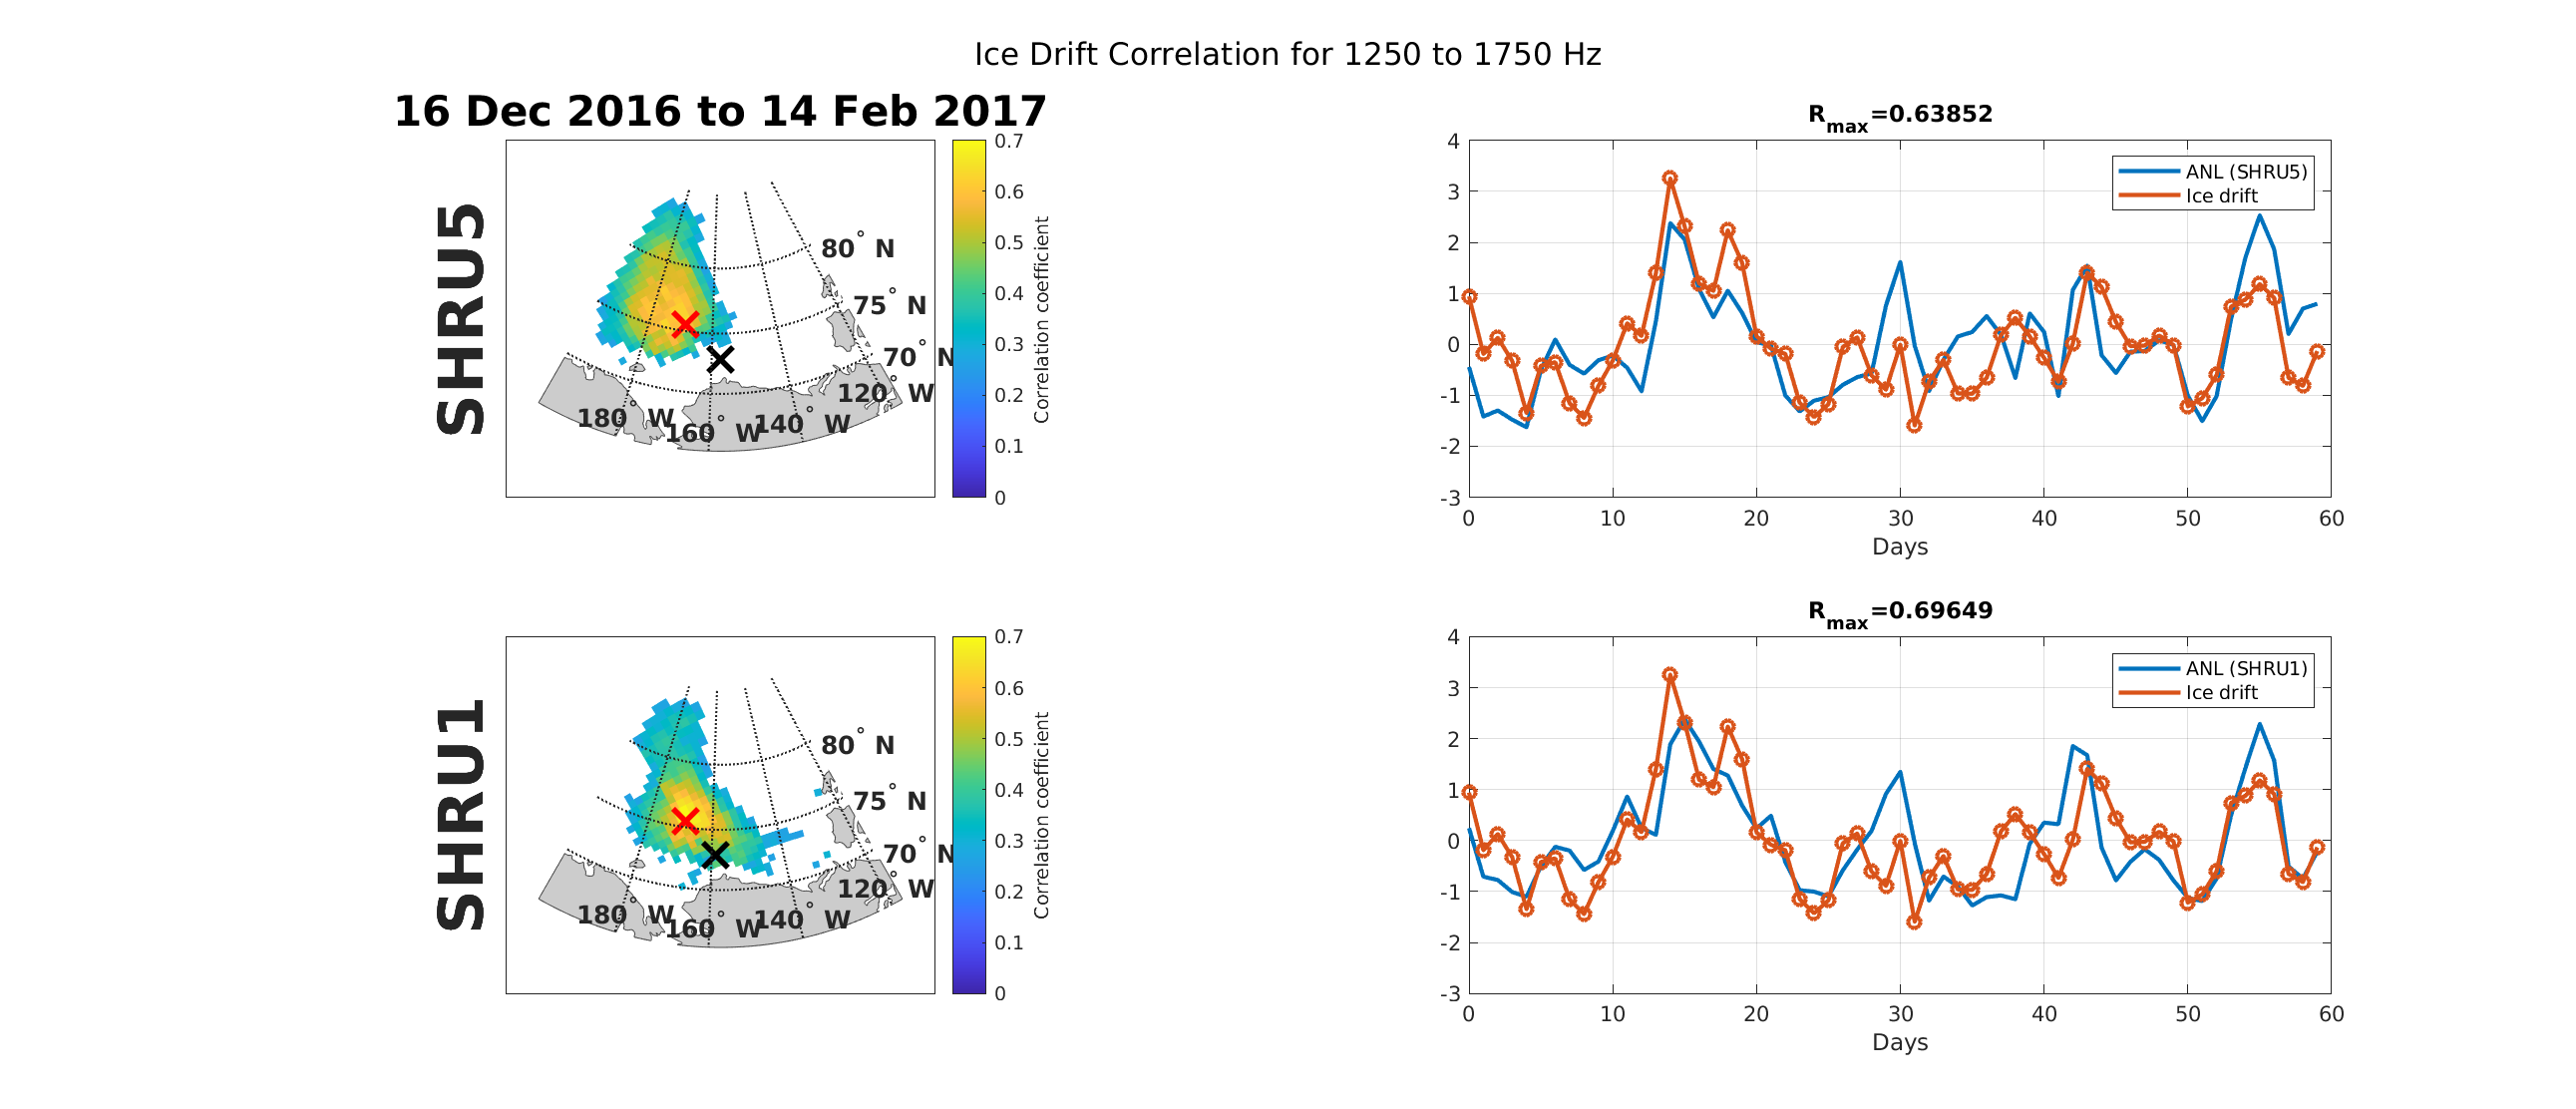
\includegraphics[scale=0.4]{Figures/spatial_corr_20161216-20170214.png}
\caption{Spacial Correlation for 1500 Hz DEC2016-JAN2017}
\label{fig_1500corr}
\end{figure}


%%%%%%%%%%%%%%%%%%%%%%%%%%%%%%%%%%%%%%%%%%%%%%%%%%%%%%%%%%%%%%%%%%%%%%%%%%
\subsection{Spacial Correlation Distance Anomaly}
\textbf{reminder: this one has the super high distance}
\textbf{Description}
This is the figure that has the wildly far away correlation, on top labeled SHRU5. 
The top row of this figure is the correlation between SHRU5 and ice drift, the bottom row is for the correlation between SHRU1 and ice drift
The only correlation values that are plotted on the left side are those with a p-value of less than {$5\%$}, signifying they are statistically significant. Anything else was simply removed 

\textbf{Analysis}
There are missing data points for the ice drift of SHRU1 which is why we’re not going to use this one
The red x for SHRU1 is much closer but the ice data is the same in terms of correlation dispersion

\textbf{What does this Mean?}
As said in the analysis above, these figures demonstrate a fairly strong correlation between the ambient noise level at 1500 Hz and the drift of ice

\textit{small pvalues are good, it says there a X\% chance that a thing happening is NOT random (reject the null hypothesis)}

%%%%%%%%%%%%%%%%%%%%%%%%%%%%%%%%%%%%%%%%%%%%%%%%%%%%%%%%%%%%%%%%%%%%%%%%%%
\subsection{Spatial Correlation Between ice drift spread and SHRU5}

\textbf{Description}
CAN I MAKE THIS BETTER IN TIME
This is an image of the  maximum spatial correlation for the frequencies from 300 Hertz to 1500 Hertz. 50 hz was intentionally left out as it simply looks bad compared to the others
correlation is denoted by the color intensity of the dot, note that there may be multiple dots in one area overlapping each other, such as the time periods on the left, there's more on the right
Frequency can be denoted by the color of the line connecting the dots as well as the edge around the dots
There is no scale for time shown on this graph, looking at individual stop shots in time shows us that the general pattern of Max correlation is to move from west to east or left to right in the image. A general interpretation of leftmost point is 2016 and rightmost point is 2017. I wish there was a way to label the points.  

\textbf{Analysis}
Remove from left to right there appears to be darker and larger, the noting that there is more correlation in between the ambient noise level and Ice movement at this time

\textbf{What does this Mean?}
At the most basic level, ice movement correlates with noise
And the general movement is from west to east


% pperhaps introduct the plane source tl equation?
\begin{figure}[h]
\centering
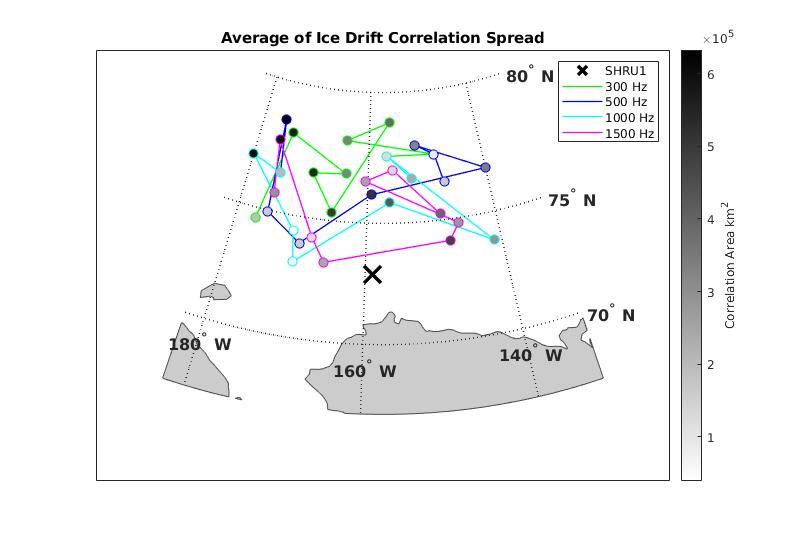
\includegraphics[scale=0.5]{Figures/avg_map_grayscale.jpg}
\caption{Average point of spatial correlation spread and area size for frequencies 300-1500 Hz}
\label{fig_maxcorr_location}
\end{figure}

%%%%%%%%%%%%%%%%%%%%%%%%%%%%%%%%%%%%%%%%%%%%%%%%%%%%%%%%%%%%%%%%%%%%%%%%%%
\subsection{Area of Correlation Spread and Maximum  through time}
\textbf{Description}
This is an image showing the distance between in the maximum correlation and SHRU5 per time instance per frequency
The x axis is date, where the length of each time period covered is two months, and there is about of month of overlap between the points.,
HIGH PINK DOT is 758 km, note SHUR1’s correlation is much closer than SHRU5, appx 150 km, this is just the point of highest correlation

\textbf{Analysis}
It would seem that higher (darker) correlation values correspond with shorter distances below 500 km, while low correlation corresponds with higher differences.
It makes sense that the 50 Hz correlations would be so high, but the pink 15000 Hz correlation doesn’t make much sense

\textbf{What does this Mean?}
There seems to be more correlation when closer to the hydrophone itself and in time, the max correlation point of the drift moves closer to the hydrophone and then away
This is NOT where the sound is coming from, this is the point of highest correlation between ice drift and ANL

\begin{figure}[h]
\centering
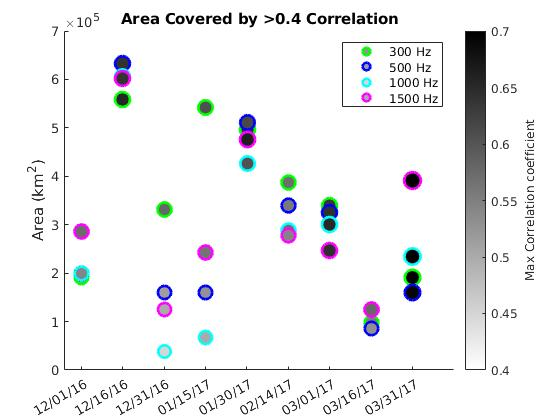
\includegraphics[scale=0.5]{Figures/area_cov_time_corrr.jpg}
\caption{Area of correlation spread in km$^{2}$ and corresponding maximum correlation value for frequencies 300-1500 Hz}
\label{fig_maxcorr_dist}
\end{figure}

%%%%%%%%%%%%%%%%%%%%%%%%%%%%%%%%%%%%%%%%%%%%%%%%%%%%%%%%%%%%%%%%%%%%%%
\subsection{Ice Correlation}
%%%%%%%%%%%%%%%%%%%%%%%%%%%%%%%%%%%%%%%%%%%%%%%%%%%%%%%%%%%%%%%%%%%%%%%%

\begin{figure}[h]
\centering
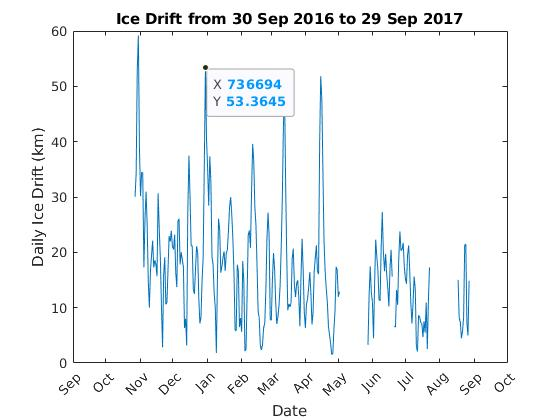
\includegraphics[scale=0.5]{Figures/sep2016_sep2017_drift.jpg}
\caption{Daily ice drift in km at SHUR5.}
\label{fig_totalice}
\end{figure}

\textbf{What is this}
this is an image of the total, non-normalized daily ice drift in kilometers from 2016Sep to 2017Sep. The highlighted dot is the second highest point of motion on 30DEC2016 with 53.36 km. The highest point occurs in 31October2016 and is 59.195 km. The ice reaches a minimum in September and reforms through October and November, so I would want to check the coverage at this point too. It may be that the drift seen in October is the ice just growing. For the December point, it is assumed that the Arctic is at full winter ice coverage. 
\textbf{What does it mean}
The ice moved a significant amount on this day in this area, so likely is was moving all over the arctic due to high winds but NEED TO VERIFY with data that I believe Julien already has somewhere. [yes there are winds] The ice got thicker from 01DEC2016 to 01JAN2017. This strong drift could be the building of the ice with a storm as well.
It cooled a bit from the 29-30 Jan 2016, from 252.6 (-20 C) K on the 27 to 245.2 (-28 C) K on the 30


\subsection{Distribution of Ice correlation}

% turn the grid on for errorbars
\begin{figure}[h]
\centering
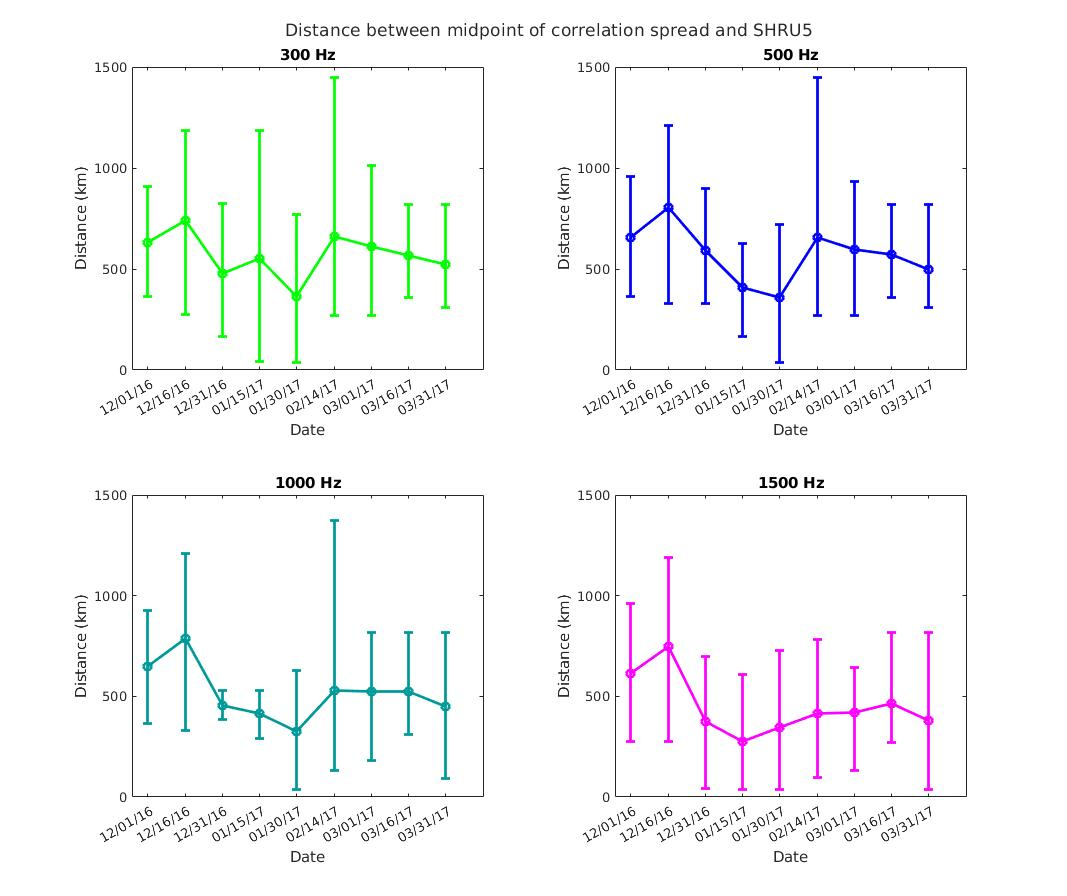
\includegraphics[scale=0.4]{Figures/errorbars_tiled.jpg}
\caption{Daily ice drift in km at SHUR5.}
\label{fig_totalice}
\end{figure}
%%%%%%%%%%%%%%%%%%%%%%%%%%%%%%%%%%%%%%%%%%%%%%%%%%%%%%%%%%%%%%%%%%%%%%%%
\section{Spacial Analysis Conclusions} %summary? conclusion? idk what to call
%%%%%%%%%%%%%%%%%%%%%%%%%%%%%%%%%%%%%%%%%%%%%%%%%%%%%%%%%%%%%%%%%%%%%%%%

%Here, sum up the 'what does this mean of the above'
%
\subsection{Correlation between Ice Drift and ANL}


%%%%%%%%%%%%%%%%%%%%%%%%%%%%%%%%%%%%%%%%%%%%%%%%%%%%%%%%%%%%%%%%%%%%%%%%

%%%%%%%%%%%%%%%%%%%%%%%%%%%%%%%%%%%%%%%%%%%%%%%%%%%%%%%%%%%%%%%%%%%%%%%%

